\documentclass[11pt]{article}
\usepackage{amsmath}
\usepackage{amssymb}
\usepackage{graphicx}
\usepackage{tabularx}
\usepackage{fancyhdr}
\usepackage{lastpage}

% Page layout
\usepackage[top=1in, bottom=1in, left=1in, right=1in]{geometry}

% Header and footer
\pagestyle{fancy}
\fancyhf{}
\rfoot{Page \thepage}
\renewcommand{\headrulewidth}{0pt}

% Modified Question command with left-aligned number
\newcommand{\questiona}[2]{
    \noindent\textbf{Q#2.} #1 \hfill \textbf{[1 Mark]}
}

\newcommand{\questionb}[2]{
    \noindent\textbf{Q#2.} #1 \hfill \textbf{[2 Marks]}
}

\begin{document}

% Title section with horizontal line
\begin{center}
    \Large\textbf{GATE 2018 - Electrical Engineering (EE)} \\
    \large\textbf{General Aptitude and Technical Questions} \\
    \rule{\textwidth}{0.5pt} % Horizontal line below heading
\end{center}

\vspace{0.5cm}

% General Aptitude Section
\section*{General Aptitude}

\questiona{Since you have gone off the \_\_\_\_\_, the \_\_\_\_\_ sand is likely to damage the car.}{1}
\begin{enumerate}
    \item[(A)] course, coarse
    \item[(B)] course, course
    \item[(C)] coarse, course
    \item[(D)] coarse, coarse
\end{enumerate}
\vspace{0.5cm}

\questiona{A common misconception among writers is that sentence structure mirrors thought; the more \_\_\_\_\_ the structure, the more complicated the ideas.}{2}
\begin{enumerate}
    \item[(A)] detailed
    \item[(B)] simple
    \item[(C)] clear
    \item[(D)] convoluted
\end{enumerate}
\vspace{0.5cm}

\questiona{The three roots of the equation \( f(x) = 0 \) are \( x = \{-2, 0, 3\} \). What are the three values of \( x \) for which \( f(x-3) = 0 \)?}{3}
\begin{enumerate}
    \item[(A)] \( -5, -3, 0 \)
    \item[(B)] \( -2, 0, 3 \)
    \item[(C)] \( 0, 6, 8 \)
    \item[(D)] \( 1, 3, 6 \)
\end{enumerate}
\vspace{0.5cm}

\questiona{For what values of \( k \) given below is \( \frac{(k+2)^2}{k-3} \) an integer?}{4}
\begin{enumerate}
    \item[(A)] 4, 8, 18
    \item[(B)] 4, 10, 16
    \item[(C)] 4, 8, 28
    \item[(D)] 8, 26, 28
\end{enumerate}
\vspace{0.5cm}

\questiona{Functions \( F(a, b) \) and \( G(a, b) \) are defined as follows: \\
\( F(a, b) = (a - b)^2 \) and \( G(a, b) = |a - b| \), where \( |x| \) represents the absolute value of \( x \). \\
What would be the value of \( G(F(1, 3), G(1, 3)) \)?}{5}
\begin{enumerate}
    \item[(A)] 2
    \item[(B)] 4
    \item[(C)] 6
    \item[(D)] 36
\end{enumerate}
\vspace{0.5cm}

\questionb{An e-mail password must contain three characters. The password has to contain one numeral from 0 to 9, one upper case and one lower case character from the English alphabet. How many distinct passwords are possible?}{6}
\begin{enumerate}
    \item[(A)] 6,760
    \item[(B)] 13,520
    \item[(C)] 40,560
    \item[(D)] 1,05,456
\end{enumerate}
\vspace{0.5cm}

\questionb{In a certain code, AMCF is written as EQGJ and NKUF is written as ROYJ. How will DHLP be written in that code?}{7}
\begin{enumerate}
    \item[(A)] RSTN
    \item[(B)] TLPH
    \item[(C)] HLPT
    \item[(D)] XSVR
\end{enumerate}
\vspace{0.5cm}

\questionb{A class of twelve children has two more boys than girls. A group of three children are randomly picked from this class to accompany the teacher on a field trip. What is the probability that the group accompanying the teacher contains more girls than boys?}{8}
\vspace{0.5cm}

\questionb{A designer uses marbles of four different colours for his designs. The cost of each marble is the same, irrespective of the colour. The table below shows the percentage of marbles of each colour used in the current design. The cost of each marble increased by 25\%. Therefore, the designer decided to reduce equal numbers of marbles of each colour to keep the total cost unchanged. What is the percentage of blue marbles in the new design?}{9}
\begin{center}
\begin{tabular}{|c|c|c|c|}
\hline
Blue & Black & Red & Yellow \\
\hline
40\% & 25\% & 20\% & 15\% \\
\hline
\end{tabular}
\end{center}
\begin{enumerate}
    \item[(A)] 35.75
    \item[(B)] 40.25
    \item[(C)] 43.75
    \item[(D)] 46.25
\end{enumerate}
\vspace{0.5cm}

\questionb{P, Q, R and S crossed a lake in a boat that can hold a maximum of two persons, with only one set of oars. The following additional facts are available. \\
(i) The boat held two persons on each of the three forward trips across the lake and one person on each of the two return trips. \\
(ii) P is unable to row when someone else is in the boat. \\
(iii) Q is unable to row with anyone else except R. \\
(iv) Each person rowed for at least one trip. \\
(v) Only one person can row during a trip. \\
Who rowed twice?}{10}
\begin{enumerate}
    \item[(A)] P
    \item[(B)] Q
    \item[(C)] R
    \item[(D)] S
\end{enumerate}
\vspace{0.5cm}

\section*{Technical Section}

\questiona{A single-phase 100 kVA, 1000 V / 100 V, 50 Hz transformer has a voltage drop of 5\% across its series impedance at full load. Of this, 3\% is due to resistance. The percentage regulation of the transformer at full load with 0.8 lagging power factor is}{1}
\begin{enumerate}
    \item[(A)] 4.8
    \item[(B)] 6.8
    \item[(C)] 8.8
    \item[(D)] 10.8
\end{enumerate}
\vspace{0.5cm}

\questiona{In a salient pole synchronous motor, the developed reluctance torque attains the maximum value when the load angle in electrical degrees is}{2}
\begin{enumerate}
    \item[(A)] 0
    \item[(B)] 45
    \item[(C)] 60
    \item[(D)] 90
\end{enumerate}
\vspace{0.5cm}

\questiona{A single phase fully controlled rectifier is supplying a load with an anti-parallel diode as shown in the figure. All switches and diodes are ideal. Which one of the following is true for instantaneous load voltage and current?}{3}
\begin{center}
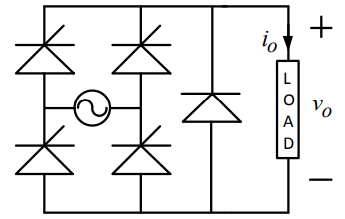
\includegraphics[width=0.5\textwidth]{figures/3.png}
\end{center}
\begin{enumerate}
    \item[(A)] \( v \geq 0 \) and \( i < 0 \)
    \item[(B)] \( v < 0 \) and \( i < 0 \)
    \item[(C)] \( v \geq 0 \) and \( i \geq 0 \)
    \item[(D)] \( v < 0 \) and \( i \geq 0 \)
\end{enumerate}
\vspace{0.5cm}

\questiona{Four power semiconductor devices are shown in the figure along with their relevant terminals. The device(s) that can carry dc current continuously in the direction shown when gated appropriately is (are)}{4}
\begin{center}
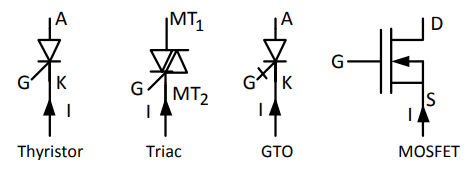
\includegraphics[width=0.5\textwidth]{figures/4.png}
\end{center}
\begin{enumerate}
    \item[(A)] Triac only
    \item[(B)] Triac and MOSFET
    \item[(C)] Triac and GTO
    \item[(D)] Thyristor and Triac
\end{enumerate}
\vspace{0.5cm}

\questiona{Two wattmeter method is used for measurement of power in a balanced three-phase load supplied from a balanced three-phase system. If one of the wattmeters reads half of the other (both positive), then the power factor of the load is}{5}
\begin{enumerate}
    \item[(A)] 0.532
    \item[(B)] 0.632
    \item[(C)] 0.707
    \item[(D)] 0.866
\end{enumerate}
\vspace{0.5cm}

\questiona{Consider a lossy transmission line with \( V_1 \) and \( V_2 \) as the sending and receiving end voltages, respectively. \( Z \) and \( X \) are the series impedance and reactance of the line, respectively. The steady-state stability limit for the transmission line will be}{6}
\begin{enumerate}
    \item[(A)] greater than \( \frac{V_1 V_2}{X} \)
    \item[(B)] less than \( \frac{V_1 V_2}{X} \)
    \item[(C)] equal to \( \frac{V_1 V_2}{X} \)
    \item[(D)] equal to \( \frac{V_1 V_2}{Z} \)
\end{enumerate}
\vspace{0.5cm}

\questiona{The graph of a network has 8 nodes and 5 independent loops. The number of branches of the graph is}{7}
\begin{enumerate}
    \item[(A)] 11
    \item[(B)] 12
    \item[(C)] 13
    \item[(D)] 14
\end{enumerate}
\vspace{0.5cm}

\questiona{In the figure, the voltages are \( v_1(t) = 100 \cos(\omega t) \), \( v_2(t) = 100 \cos(\omega t + \pi/18) \) and \( v_3(t) = 100 \cos(\omega t + \pi/36) \). The circuit is in sinusoidal steady state, and \( R \ll \omega L \). \( P_1, P_2 \) and \( P_3 \) are the average power outputs. Which one of the following statements is true?}{8}
\begin{center}
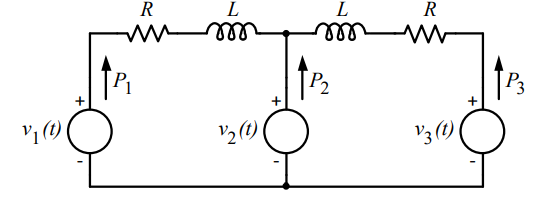
\includegraphics[width=0.5\textwidth]{figures/8.png}
\end{center}
\begin{enumerate}
    \item[(A)] \( P_1 = P_2 = P_3 = 0 \)
    \item[(B)] \( P_1 < 0, P_2 > 0, P_3 > 0 \)
    \item[(C)] \( P_1 < 0, P_2 > 0, P_3 < 0 \)
    \item[(D)] \( P_1 > 0, P_2 < 0, P_3 > 0 \)
\end{enumerate}
\vspace{0.5cm}

\questiona{Match the transfer functions of the second-order systems with the nature of the systems given below. \\
\textbf{Transfer functions} \\
P: \( \frac{15}{s^2 + 5s + 15} \) \\
Q: \( \frac{25}{s^2 + 10s + 25} \) \\
R: \( \frac{35}{s^2 + 18s + 35} \) \\
\textbf{Nature of system} \\
I: Overdamped \hspace{0.5cm} II: Critically damped \hspace{0.5cm} III: Underdamped}{9}
\begin{enumerate}
    \item[(A)] P-I, Q-II, R-III
    \item[(B)] P-II, Q-I, R-III
    \item[(C)] P-III, Q-II, R-I
    \item[(D)] P-III, Q-I, R-II
\end{enumerate}
\vspace{0.5cm}

\questiona{A positive charge of 1 nC is placed at (0, 0, 0.2) where all dimensions are in metres. Consider the \( x\text{-}y \) plane to be a conducting ground plane. Take \( \varepsilon_0 = 8.85 \times 10^{-12} \text{ F/m} \). The \( z \)-component of the electric field at (0, 0, 0.1) is closest to}{10}
\begin{enumerate}
    \item[(A)] 899.18 V/m
    \item[(B)] –899.18 V/m
    \item[(C)] 999.09 V/m
    \item[(D)] –999.09 V/m
\end{enumerate}
\vspace{0.5cm}

\questiona{Let \( f \) be a real-valued function of a real variable defined as \( f(x) = x^2 \) for \( x \geq 0 \), and \( f(x) = -x^2 \) for \( x < 0 \). Which one of the following statements is true?}{11}
\begin{enumerate}
    \item[(A)] \( f(x) \) is discontinuous at \( x = 0 \)
    \item[(B)] \( f(x) \) is continuous but not differentiable at \( x = 0 \)
    \item[(C)] \( f(x) \) is differentiable but its first derivative is not continuous at \( x = 0 \)
    \item[(D)] \( f(x) \) is differentiable but its first derivative is not differentiable at \( x = 0 \)
\end{enumerate}
\vspace{0.5cm}

\questiona{The value of the directional derivative of the function \( \Phi(x, y, z) = xy^2 + yz^2 + zx^2 \) at the point (2, –1, 1) in the direction of the vector \( \mathbf{p} = \hat{i} + 2\hat{j} + 2\hat{k} \) is}{12}
\begin{enumerate}
    \item[(A)] 1
    \item[(B)] 0.95
    \item[(C)] 0.93
    \item[(D)] 0.9
\end{enumerate}
\vspace{0.5cm}

\questiona{The value of the integral \( \oint \frac{z+1}{z^2 - 4} \, dz \) in counter-clockwise direction around a circle \( C \) of radius 1 with center at the point \( z = -2 \) is}{13}
\begin{enumerate}
    \item[(A)] \( \frac{\pi i}{2} \)
    \item[(B)] \( 2\pi i \)
    \item[(C)] \( -\frac{\pi i}{2} \)
    \item[(D)] \( -2\pi i \)
\end{enumerate}
\vspace{0.5cm}

\questiona{In the logic circuit shown in the figure, \( Y \) is given by}{14}
\begin{center}
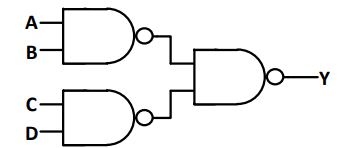
\includegraphics[width=0.5\textwidth]{figures/14.png}
\end{center}
\begin{enumerate}
    \item[(A)] \( Y = ABCD \)
    \item[(B)] \( Y = (A + B)(C + D) \)
    \item[(C)] \( Y = A + B + C + D \)
    \item[(D)] \( Y = AB + CD \)
\end{enumerate}
\vspace{0.5cm}

\questiona{The op-amp shown in the figure is ideal. The input impedance \( \frac{v_{\text{in}}}{i_{\text{in}}} \) is given by}{15}
\begin{center}
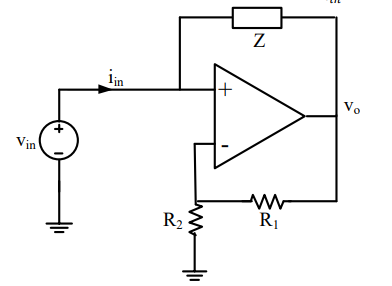
\includegraphics[width=0.5\textwidth]{figures/15.png}
\end{center}
\begin{enumerate}
    \item[(A)] \( Z \frac{R_1}{R_2} \)
    \item[(B)] \( -Z \frac{R_2}{R_1} \)
    \item[(C)] \( Z \)
    \item[(D)] \( -Z \frac{R_1}{R_1 + R_2} \)
\end{enumerate}
\vspace{0.5cm}

\questiona{A continuous-time input signal \( x(t) \) is an eigenfunction of an LTI system, if the output is}{16}
\begin{enumerate}
    \item[(A)] \( k x(t) \), where \( k \) is an eigenvalue
    \item[(B)] \( k e^{j\omega t} x(t) \), where \( k \) is an eigenvalue and \( e^{j\omega t} \) is a complex exponential signal
    \item[(C)] \( x(t) e^{j\omega t} \), where \( e^{j\omega t} \) is a complex exponential signal
    \item[(D)] \( k H(\omega) \), where \( k \) is an eigenvalue and \( H(\omega) \) is a frequency response of the system
\end{enumerate}
\vspace{0.5cm}

\questiona{Consider a non-singular \( 2 \times 2 \) square matrix \( A \). If \( \text{trace}(A) = 4 \) and \( \text{trace}(A^2) = 5 \), the determinant of the matrix \( A \) is}{17}
\vspace{0.5cm}

\questiona{Let \( f(x) = x - [x] \), where \( [x] \) denotes the greatest integer less than or equal to \( x \). The value of \( \int_{0.25}^{1.25} f(x) \, dx \) is}{18}
\vspace{0.5cm}

\questiona{In the two-port network shown, the \( h_{11} \) parameter is given by \( h_{11} = \left. \frac{V_1}{I_1} \right|_{V_2=0} \). The value in ohms is}{19}
\begin{center}
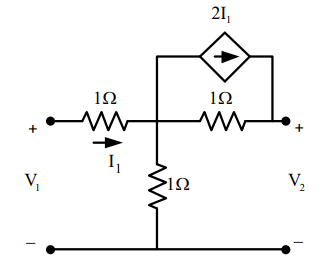
\includegraphics[width=0.5\textwidth]{figures/19.png}
\end{center}
\vspace{0.5cm}

\questiona{The series impedance matrix of a short three-phase transmission line in phase coordinates is
\[
\begin{bmatrix}
Z_s & Z_m & Z_m \\
Z_m & Z_s & Z_m \\
Z_m & Z_m & Z_s
\end{bmatrix}.
\]
If the positive sequence impedance is \( (1 + j10)~\Omega \), and the zero sequence is \( (4 + j31)~\Omega \), then the imaginary part of \( Z_m \) (in \( \Omega \)) is}{20}
\vspace{0.5cm}

\questiona{The positive, negative and zero sequence impedances of a 125 MVA, three-phase, 15.5 kV, star-grounded, 50 Hz generator are \( j0.1 \, \text{pu}, j0.05 \, \text{pu} \) and \( j0.01 \, \text{pu} \) respectively on the machine rating base. The machine is unloaded and working at the rated terminal voltage. If the grounding impedance of the generator is \( j0.01 \, \text{pu} \), then the magnitude of fault current for a b-phase to ground fault (in kA) is}{21}
\vspace{0.5cm}

\questiona{A \( 1000 \times 1000 \) bus admittance matrix for an electric power system has 8000 non-zero elements. The minimum number of branches (transmission lines and transformers) in this system are}{22}
\vspace{0.5cm}

\questiona{The waveform of the current drawn by a semi-converter from a sinusoidal AC voltage source is shown in the figure. If \( I_0 = 20 \) A, the rms value of fundamental component of the current is}{23}
\begin{center}
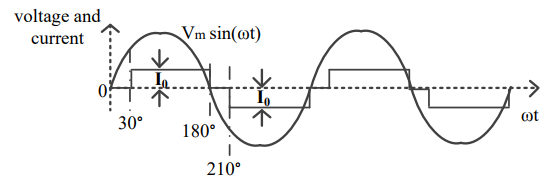
\includegraphics[width=0.5\textwidth]{figures/23.png}
\end{center}
\vspace{0.5cm}

\questiona{A separately excited dc motor has an armature resistance \( R_a = 0.05 \, \Omega \). The field excitation is kept constant. At an armature voltage of 100 V, the motor produces a torque of 500 Nm at zero speed. Neglecting all mechanical losses, the no-load speed of the motor (in radian/s) for an armature voltage of 150 V is}{24}
\vspace{0.5cm}

\questiona{Consider a unity feedback system with forward transfer function given by \( G(s) = \frac{1}{(s+1)(s+2)} \). The steady-state error in the output of the system for a unit-step input is}{25}
\vspace{0.5cm}

\questionb{A transformer with toroidal core of permeability \( \mu \) is shown in the figure. Assuming uniform flux density across the circular core cross-section of radius \( r \ll R \), and neglecting any leakage flux, the best estimate for the mean radius \( R \) is}{26}
\begin{center}
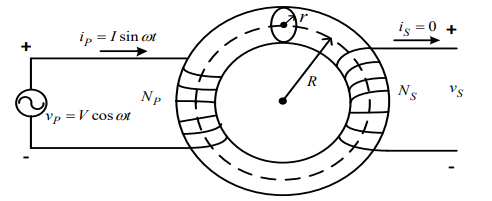
\includegraphics[width=0.5\textwidth]{figures/26.png}
\end{center}
\begin{enumerate}
    \item[(A)] \( \frac{2P V r^2 N}{I \mu \omega} \)
    \item[(B)] \( \frac{2P I r^2 N}{V \mu \omega} \)
    \item[(C)] \( \frac{P V r^2 N}{I \mu \omega} \)
    \item[(D)] \( \frac{P I r^2 N}{V \mu \omega} \)
\end{enumerate}
\vspace{0.5cm}

\questionb{A 0–1 Ampere moving iron ammeter has an internal resistance of \( 50 \, \text{m}\Omega \) and inductance of 0.1 mH. A shunt coil is connected to extend its range to 0–10 Ampere for all operating frequencies. The time constant in milliseconds and resistance in mΩ of the shunt coil respectively are}{27}
\begin{enumerate}
    \item[(A)] 2, 5.55
    \item[(B)] 2, 1
    \item[(C)] 2.18, 0.55
    \item[(D)] 11.1, 2
\end{enumerate}
\vspace{0.5cm}

\questionb{The positive, negative and zero sequence impedances of a three-phase generator are \( Z_1, Z_2 \) and \( Z_0 \) respectively. For a line-to-line fault with fault impedance \( Z_f \), the fault current is \( I_{f1} = k I_f \), where \( I_f \) is the fault current with zero fault impedance. The relation between \( Z_f \) and \( k \) is}{28}
\begin{enumerate}
    \item[(A)] \( Z_f = \frac{(Z_1 + Z_2)(1 - k)}{k} \)
    \item[(B)] \( Z_f = \frac{(Z_1 + Z_2)(1 + k)}{k} \)
    \item[(C)] \( Z_f = \frac{(Z_1 + Z_2)k}{1 - k} \)
    \item[(D)] \( Z_f = \frac{(Z_1 + Z_2)k}{1 + k} \)
\end{enumerate}
\vspace{0.5cm}

\questionb{Consider the two bus power system network with given loads as shown in the figure. All the values shown in the figure are in per unit. The reactive power supplied by generator \( G_1 \) and \( G_2 \) are \( Q_{G1} \) and \( Q_{G2} \) respectively. The per unit values of \( Q_{G1}, Q_{G2} \), and line reactive power loss \( Q_{\text{loss}} \) respectively are}{29}
\begin{center}
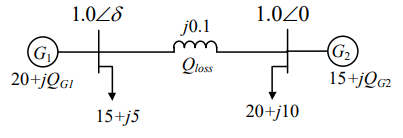
\includegraphics[width=0.5\textwidth]{figures/29.png}
\end{center}
\begin{enumerate}
    \item[(A)] 5.00, 12.68, 2.68
    \item[(B)] 6.34, 10.00, 1.34
    \item[(C)] 6.34, 11.34, 2.68
    \item[(D)] 5.00, 11.34, 1.34
\end{enumerate}
\vspace{0.5cm}

\questionb{The per-unit power output of a salient-pole generator which is connected to an infinite bus, is given by the expression, \( P = 1.4 \sin \delta + 0.15 \sin 2\delta \), where \( \delta \) is the load angle. Newton-Raphson method is used to calculate the value of \( \delta \) for \( P = 0.8 \, \text{pu} \). If the initial guess is \( 30^\circ \), then its value (in degrees) at the end of the first iteration is}{30}
\begin{enumerate}
    \item[(A)] \( 15^\circ \)
    \item[(B)] \( 28.48^\circ \)
    \item[(C)] \( 28.74^\circ \)
    \item[(D)] \( 31.20^\circ \)
\end{enumerate}
\vspace{0.5cm}

\questionb{A DC voltage source is connected to a series L-C circuit by turning on the switch \( S \) at time \( t = 0 \) as shown in the figure. Assume \( i(0) = 0 \), \( v(0) = 0 \). Which one of the following circular loci represents the plot of \( i(t) \) versus \( v(t) \)?}{31}
\begin{center}
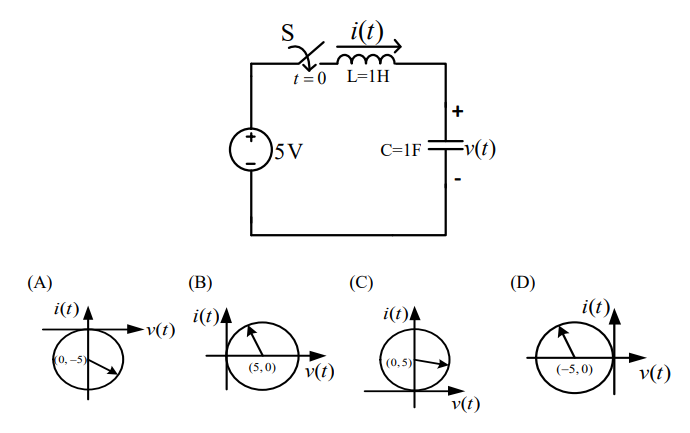
\includegraphics[width=1\textwidth]{figures/31.png}
\end{center}

\vspace{0.5cm}

\questionb{The equivalent impedance \( Z_{\text{eq}} \) for the infinite ladder circuit shown in the figure is}{32}
\begin{center}
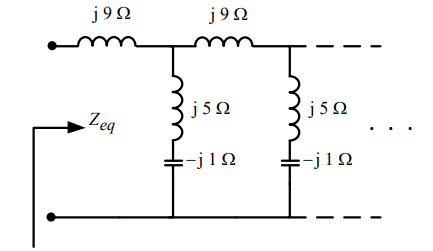
\includegraphics[width=0.5\textwidth]{figures/32.png}
\end{center}
\begin{enumerate}
    \item[(A)] \( j12 \, \Omega \)
    \item[(B)] \( -j12 \, \Omega \)
    \item[(C)] \( j13 \, \Omega \)
    \item[(D)] \( 13 \, \Omega \)
\end{enumerate}
\vspace{0.5cm}

\questionb{Consider a system governed by the following equations: \\
\[
\frac{dx_1(t)}{dt} = -x_1(t)x_2(t), \quad \frac{dx_2(t)}{dt} = x_1(t) - x_2(t)
\] \\
The initial conditions are such that \( 0 < x_1(0) < x_2(0) < \infty \). Let \( f_1 = \lim_{t \to \infty} x_1(t) \) and \( f_2 = \lim_{t \to \infty} x_2(t) \). Which one of the following is true?}{33}
\begin{enumerate}
    \item[(A)] \( 0 < f_1 < f_2 < \infty \)
    \item[(B)] \( 0 < f_2 < f_1 < \infty \)
    \item[(C)] \( 0 < f_1 = f_2 < \infty \)
    \item[(D)] \( f_1 = f_2 = \infty \)
\end{enumerate}
\vspace{0.5cm}

\questionb{The number of roots of the polynomial \( s^7 + s^6 + 7s^5 + 14s^4 + 31s^3 + 73s^2 + 25s + 200 \) in the open left half of the complex plane is}{34}
\begin{enumerate}
    \item[(A)] 3
    \item[(B)] 4
    \item[(C)] 5
    \item[(D)] 6
\end{enumerate}
\vspace{0.5cm}

\questionb{If \( C \) is a circle \( |z| = 4 \) and \( f(z) = \frac{z^2}{(z^2 - 3z + 2)^2} \), then \( \oint_C f(z) \, dz \) is}{35}
\begin{enumerate}
    \item[(A)] 1
    \item[(B)] 0
    \item[(C)] –1
    \item[(D)] –2
\end{enumerate}
\vspace{0.5cm}

\questionb{Which one of the following statements is true about the digital circuit shown in the figure?}{36}
\begin{center}
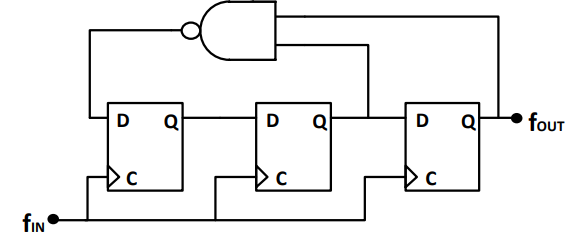
\includegraphics[width=0.5\textwidth]{figures/36.png}
\end{center}
\begin{enumerate}
    \item[(A)] It can be used for dividing the input frequency by 3.
    \item[(B)] It can be used for dividing the input frequency by 5.
    \item[(C)] It can be used for dividing the input frequency by 7.
    \item[(D)] It cannot be reliably used as a frequency divider due to disjoint internal cycles.
\end{enumerate}
\vspace{0.5cm}

\questionb{Digital input signals \( A, B, C \) with \( A \) as the MSB and \( C \) as the LSB are used to realize the Boolean function \( F = m_0 + m_2 + m_3 + m_5 + m_7 \), where \( m_i \) denotes the \( i^{th} \) minterm. In addition, \( F \) has a don’t care for \( m_1 \). The simplified expression for \( F \) is given by}{37}
\begin{enumerate}
    \item[(A)] \( \bar{A}\bar{B}\bar{C} + \bar{A}\bar{B}C + AC \)
    \item[(B)] \( \bar{A}\bar{B} + C \)
    \item[(C)] \( \bar{C} + A \)
    \item[(D)] \( \bar{A}\bar{B}C + BC + A\bar{C} \)
\end{enumerate}
\vspace{0.5cm}

\questionb{Consider the two continuous-time signals defined below:
\[
x_1(t) = \begin{cases}
1, & -1 \leq t \leq 1 \\
0, & \text{otherwise}
\end{cases}, \quad
x_2(t) = \begin{cases}
2 - t, & 1 \leq t \leq 2 \\
0, & \text{otherwise}
\end{cases}
\]
These signals are sampled with a sampling period of \( T = 0.25 \) seconds to obtain discrete-time signals \( x_1[n] \) and \( x_2[n] \), respectively. Which one of the following statements is true?}{38}
\begin{enumerate}
    \item[(A)] The energy of \( x_1[n] \) is greater than the energy of \( x_2[n] \).
    \item[(B)] The energy of \( x_2[n] \) is greater than the energy of \( x_1[n] \).
    \item[(C)] \( x_1[n] \) and \( x_2[n] \) have equal energies.
    \item[(D)] Neither \( x_1[n] \) nor \( x_2[n] \) is a finite-energy signal.
\end{enumerate}
\vspace{0.5cm}

\questionb{The signal energy of the continuous-time signal \( x(t) = [(1 - t)u(1 - t)] + [-(2 - t)u(2 - t)] + [-(3 - t)u(3 - t)] + [(4 - t)u(4 - t)] \) is}{39}
\begin{enumerate}
    \item[(A)] \( \frac{11}{3} \)
    \item[(B)] \( \frac{7}{3} \)
    \item[(C)] \( \frac{1}{3} \)
    \item[(D)] \( \frac{5}{3} \)
\end{enumerate}
\vspace{0.5cm}

\questionb{The Fourier transform of a continuous-time signal \( x(t) \) is given by \( X(\omega) = \frac{1}{1 + j2\omega} \), where \( \omega \) denotes frequency. Then the value of \( \ln(x(t)) \) at \( t = 1 \) is}{40}
\vspace{0.5cm}

\questionb{In the circuit shown in the figure, the bipolar junction transistor (BJT) has a current gain \( \beta = 100 \). The base-emitter voltage drop is a constant, \( V_{BE} = 0.7 \, \text{V} \). The value of the Thevenin equivalent resistance \( R_{Th} \) (in \( \Omega \)) as shown in the figure is}{41}
\begin{center}
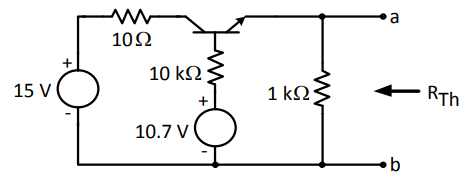
\includegraphics[width=0.5\textwidth]{figures/41.png}
\end{center}
\vspace{0.5cm}

\questionb{As shown in the figure, \( C \) is the arc from the point (3,0) to the point (0,3) on the circle \( x^2 + y^2 = 9 \). The value of the integral \( \int_C (y^2 + 2yx)\,dx + (2xy + x^2)\,dy \) is}{42}
\begin{center}
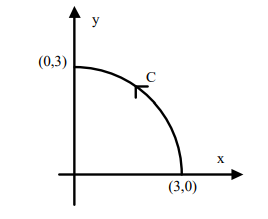
\includegraphics[width=0.5\textwidth]{figures/42.png}
\end{center}
\vspace{0.5cm}

\questionb{Let \( f(x) = 3x^3 - 7x^2 + 5x + 6 \). The maximum value of \( f(x) \) over the interval \([0, 2]\) is}{43}
\vspace{0.5cm}

\questionb{Let
\[
A = \begin{bmatrix}
1 & 0 & 1 \\
1 & 2 & 0 \\
0 & 0 & 2
\end{bmatrix}, \quad
B = 3A^3 - 2A^2 + 4A + 5I
\]
where \( I \) is the \( 3 \times 3 \) identity matrix. The determinant of \( B \) is}{44}
\vspace{0.5cm}

\questionb{The capacitance of an air-filled parallel-plate capacitor is 60 pF. When a dielectric slab whose thickness is half the distance between the plates is placed on one of the plates covering it entirely, the capacitance becomes 86 pF. Neglecting the fringing effects, the relative permittivity of the dielectric is}{45}
\vspace{0.5cm}

\questionb{The unit step response \( y(t) \) of a unity feedback system with open loop transfer function
\[
G(s)H(s) = \frac{K}{(s+1)(s+2)}
\]
is shown in the figure. The value of \( K \) is}{46}
\begin{center}
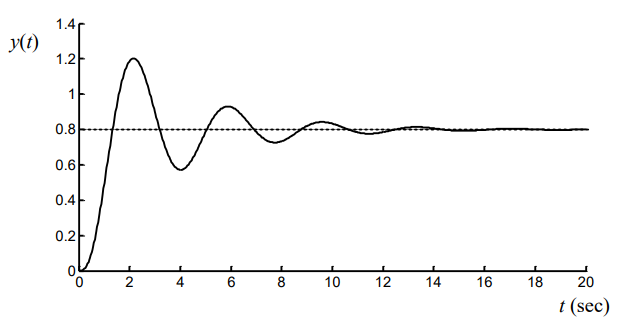
\includegraphics[width=0.5\textwidth]{figures/46.png}
\end{center}
\vspace{0.5cm}

\questionb{A three-phase load is connected to a three-phase balanced supply as shown in the figure. If \( V_{an} = 100\angle 0^\circ \, \text{V} \), \( V_{bn} = 100\angle -120^\circ \, \text{V} \), and \( V_{cn} = 100\angle -240^\circ \, \text{V} \) (angles are considered positive in the anti-clockwise direction), the value of \( R \) for zero current in the neutral wire is}{47}
\begin{center}
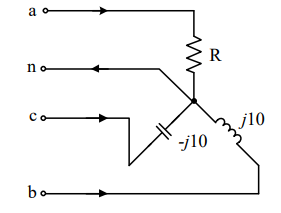
\includegraphics[width=0.5\textwidth]{figures/47.png}
\end{center}
\vspace{0.5cm}

\questionb{The voltage across the circuit in the figure, and the current through it, are given by the following expressions: \\
\( v(t) = 5 - 10 \cos(\omega t + 60^\circ) \, \text{V} \), \quad \( i(t) = 5 + X \cos(\omega t) \, \text{A} \) \\
where \( \omega = 100\pi \, \text{rad/s} \). If the average power delivered to the circuit is zero, then the value of \( X \) (in Ampere) is}{48}
\begin{center}
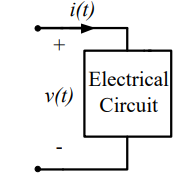
\includegraphics[width=0.5\textwidth]{figures/48.png}
\end{center}
\vspace{0.5cm}

\questionb{A phase controlled single phase rectifier, supplied by an AC source, feeds power to an \( R-L-E \) load as shown in the figure. The rectifier output voltage has an average value given by \( V_o = \frac{V_m}{2\pi}(3 + \cos \alpha) \), where \( V_m = 80\pi \, \text{V} \) and \( \alpha \) is the firing angle. If the power delivered to the lossless battery is 1600 W, \( \alpha \) in degrees is}{49}
\begin{center}
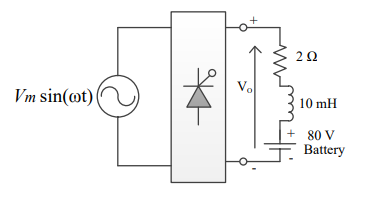
\includegraphics[width=0.5\textwidth]{figures/49.png}
\end{center}
\vspace{0.5cm}

\questionb{The figure shows two buck converters connected in parallel. The common input DC voltage for the converters has a value of 100 V. The converters have inductors of identical value. The load resistance is \( 1 \, \Omega \). The capacitor voltage has negligible ripple. Both converters operate in the continuous conduction mode. The switching frequency is 1 kHz, and the switch control signals are as shown. The circuit operates in the steady state. Assuming that the converters share the load equally, the average value of \( i_{S1} \), the current of switch \( S_1 \) (in Ampere), is}{50}
\begin{center}
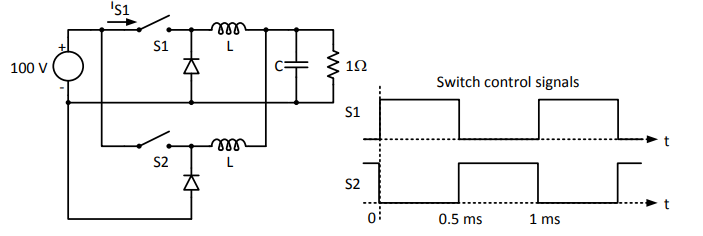
\includegraphics[width=0.8\textwidth]{figures/50.png}
\end{center}
\vspace{0.5cm}

\questionb{A 3-phase 900 kVA, 3 kV / \( \sqrt{3} \) kV (\( \Delta / Y \)), 50 Hz transformer has primary (high voltage side) resistance per phase of \( 0.3\, \Omega \) and secondary (low voltage side) resistance per phase of \( 0.02\, \Omega \). Iron loss of the transformer is 10 kW. The full load \% efficiency of the transformer operated at unity power factor is}{51}
\vspace{0.5cm}

\questionb{A 200 V DC series motor, when operating from rated voltage while driving a certain load, draws 10 A current and runs at 1000 r.p.m. The total series resistance is \( 1\, \Omega \). The magnetic circuit is assumed to be linear. At the same supply voltage, the load torque is increased by 44\%. The speed of the motor in r.p.m. (rounded to the nearest integer) is}{52}
\vspace{0.5cm}

\questionb{A DC to DC converter shown in the figure is charging a battery bank, \( B_2 \), whose voltage is constant at 150 V. \( B_1 \) is another battery bank whose voltage is constant at 50 V. The value of the inductor, \( L \), is 5 mH and the ideal switch \( S \) is operated with a switching frequency of 5 kHz with a duty ratio of 0.4. Once the circuit has attained steady state and assuming the diode \( D \) to be ideal, the power transferred from \( B_1 \) to \( B_2 \) (in Watt) is}{53}
\begin{center}
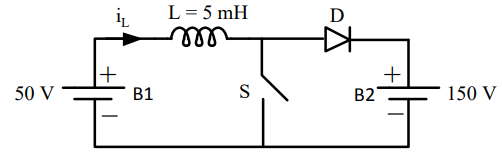
\includegraphics[width=0.5\textwidth]{figures/53.png}
\end{center}
\vspace{0.5cm}

\questionb{The equivalent circuit of a single phase induction motor is shown in the figure, where the parameters are \( R_1 = R_2' = X_{l1} = X_{l2}' = 2\, \Omega \), \( X_m = 240\, \Omega \), and \( s \) is the slip. At no-load, the motor speed can be approximated to be the synchronous speed. The no-load lagging power factor of the motor is}{54}
\begin{center}
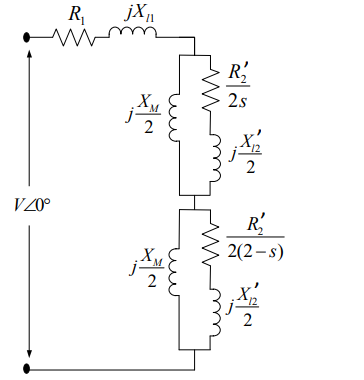
\includegraphics[width=0.5\textwidth]{figures/54.png}
\end{center}
\vspace{0.5cm}

\questionb{The voltage \( v(t) \) across the terminals \( a \) and \( b \) as shown in the figure is a sinusoidal voltage having a frequency \( \omega = 100 \, \text{rad/s} \). When the inductor current \( i(t) \) is in phase with the voltage \( v(t) \), the magnitude of the impedance \( Z \) (in \( \Omega \)) seen between the terminals \( a \) and \( b \) is}{55}
\begin{center}
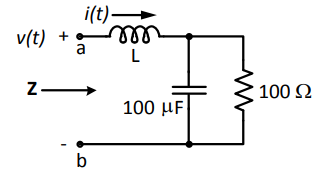
\includegraphics[width=0.5\textwidth]{figures/55.png}
\end{center}
\vspace{0.5cm}

\vspace{5cm}
\begin{center}
\textbf{END OF THE QUESTION PAPER} \\
\rule{\textwidth}{0.5pt}
\end{center}

\end{document}



\end{document}